\providecommand{\main}{../../../..}
\documentclass[\main/dresen_thesis.tex]{subfiles}
\begin{document}
  \label{sec:monolayers:nanoparticle:vsm}

  \begin{figure}[tb]
    \centering
    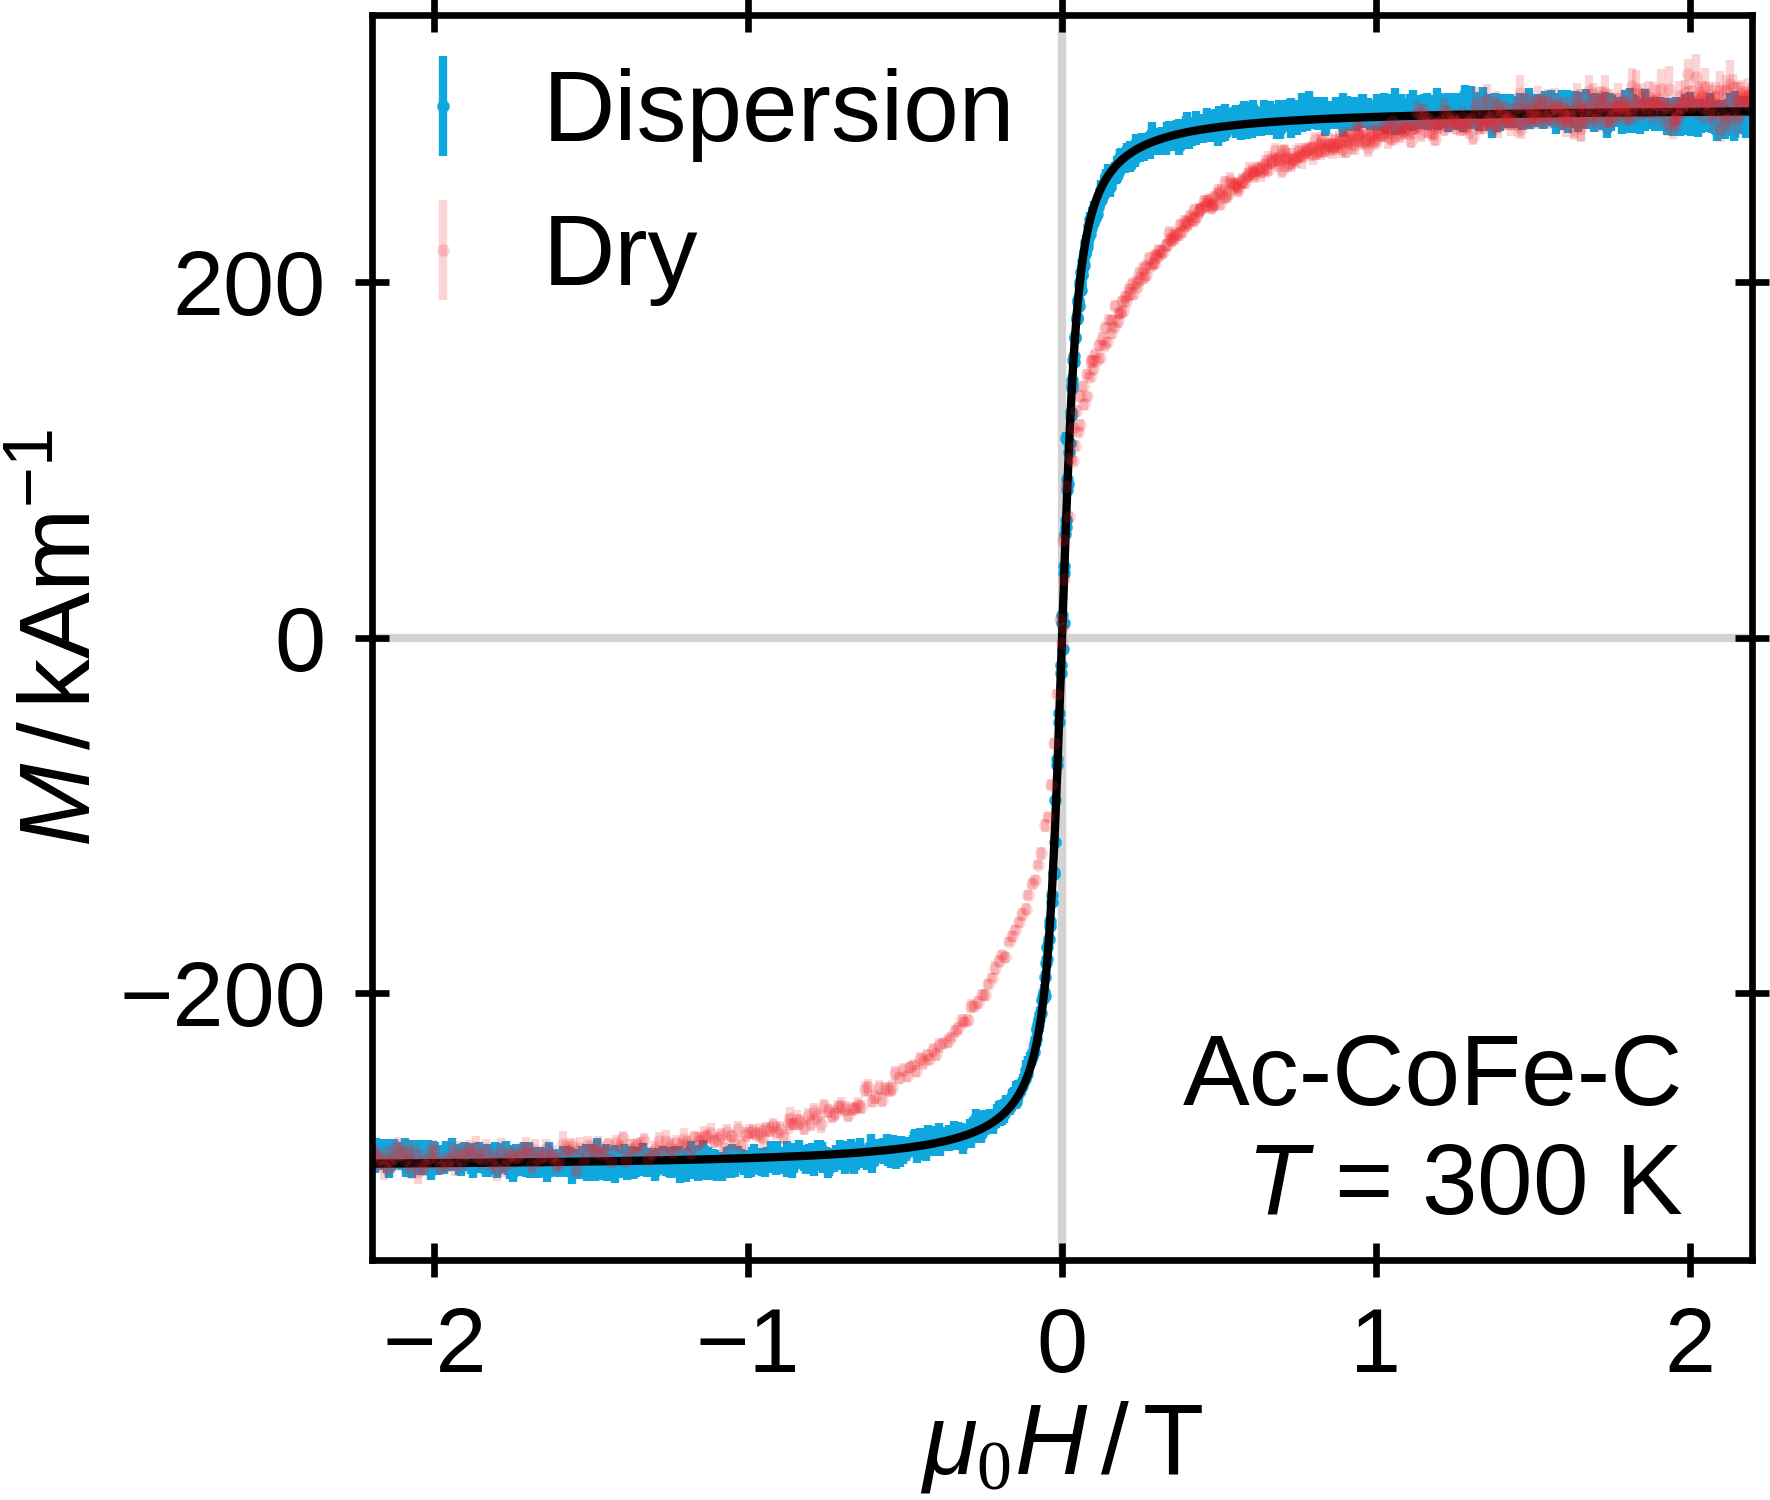
\includegraphics{monolayer_VSM_300K_Ac_CoFe_C}
    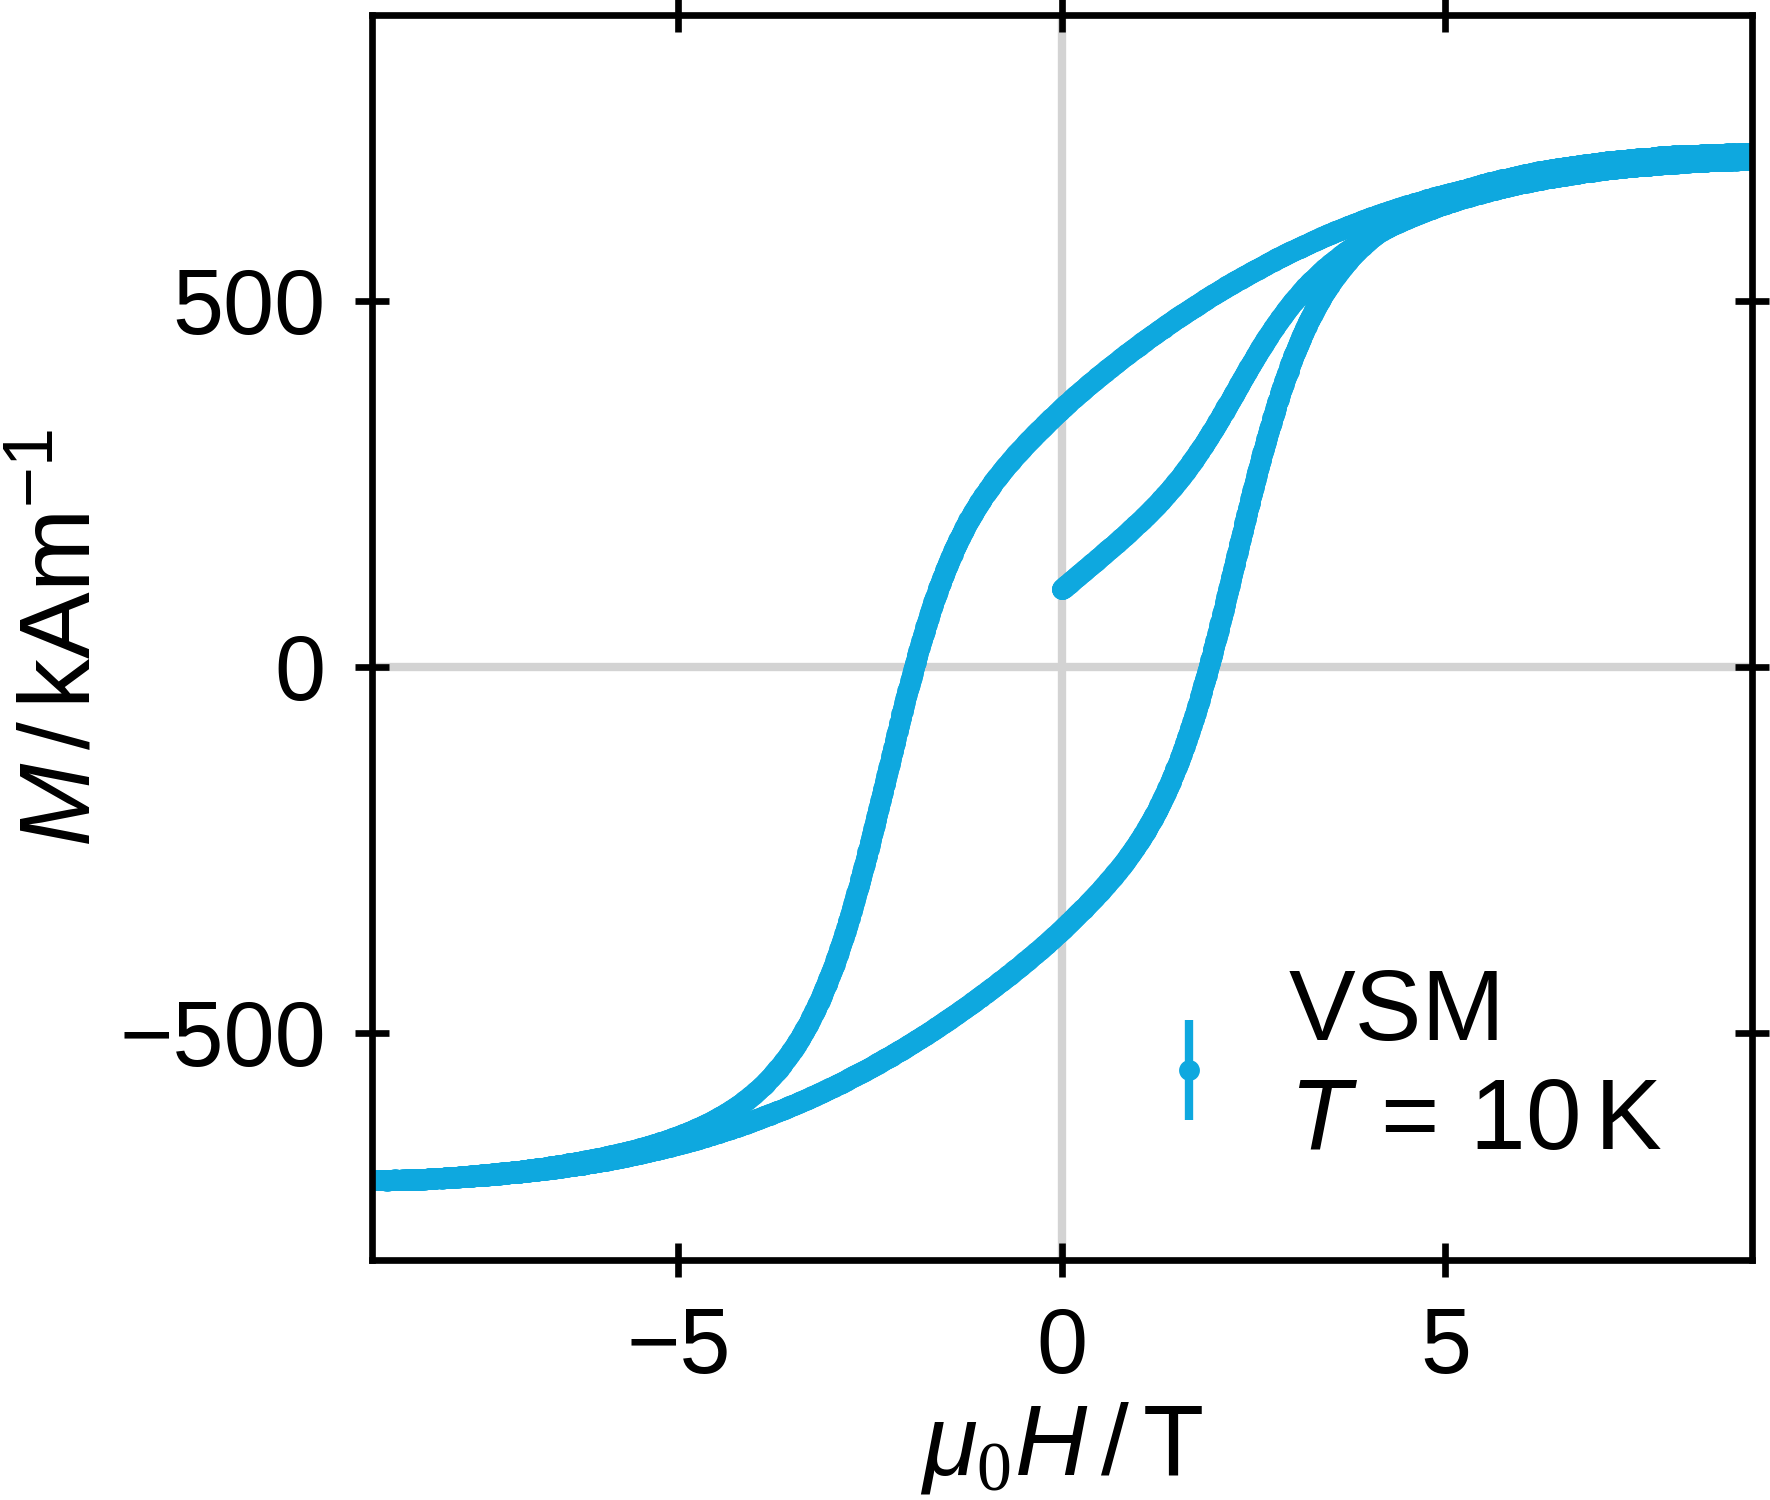
\includegraphics{monolayer_VSM_10K_Ac_CoFe_C}
    \caption{\label{fig:monolayers:nanoparticle:vsmAcCoFeC}Vibrating sample magnetometry Ac-CoFe-C at room temperature (left) and at $10 \unit{K}$ (right). The nanocubes are measured in dispersion and dried on a silicon substrate. The measurements in the dry state are corrected for the diamagnetic contribution from silicon.}
  \end{figure}

  The macroscopic field-dependent magnetization of the Ac-CoFe-C nanocubes was measured in an \textit{n}-hexane dispersion, as well as in a dry state after evaporation from \textit{n}-hexane without addends and is shown in \reffig{fig:monolayers:nanoparticle:vsmAcCoFeC}.
  At room temperature the magnetization in dispersion is well described by a Langevin behaviour.
  In a dry state, the nanocubes deviate from this behaviour at room temperature already and show a lower approach to the saturated state in direct comparison.
  The dispersion measurement is used to determine the single-particle magnetic moment to $\mu \eq 23130(80) \mu_B$.
  Using the nanocube size characterization from small-angle X-ray scattering in \refsec{sec:monolayers:nanoparticle:sas}, the spontaneous magnetization is estimated by the nanocube volume to $M_s \eq 300(5) \unit{kA\, m^{-1}}$.

  At $10 \unit{K}$, the magnetization shows a hysteretic behaviour with a coercive field of $2.0 \unit{T}$.
  Coming from a high magnetic field, the nanocubes in the frozen dispersion gradually decrease in magnetization, whereas the dried nanocubes on the substrate only start to substantially decrease in magnetization below a field of $500 \unit{mT}$.

  The different behaviour of the nanocubes in frozen dispersion and in the dry state on the wafer can be connected to the smaller interparticle distance in the dry state in comparison to the dispersion.
  From the particle concentration determined by small-angle X-ray scattering in \refsec{sec:monolayers:nanoparticle:sas}, the average interparticle spacing can be estimated to $160 \unit{nm}$ from the Wigner-Seitz radius.
  Whereas the nanocubes on the dry substrate are in close contact from the drying process and the concentration can not be reduced far below the monolayer concentration due to the finite resolution of a magnetometer.

  The measurement in dispersion does not allow to properly measure the temperature-dependent magnetization as the freezing temperature of the used organic solvent is in the order of $180 \unit{K}$ and above the nanocube magnetic behaviour is masked by Brownian motion.
  Using the nanocubes in the dry state, shown in \reffig{monolayer_PPMS_ZFC_FC_ML_Ac_CoFe_C} (left), the blocking temperature is found at a high temperature of $315 \unit{K}$.
  However, due to the small interparticle distance it must be assumed that this value is already affected by interparticle interactions.

  \begin{figure}[tb]
    \centering
    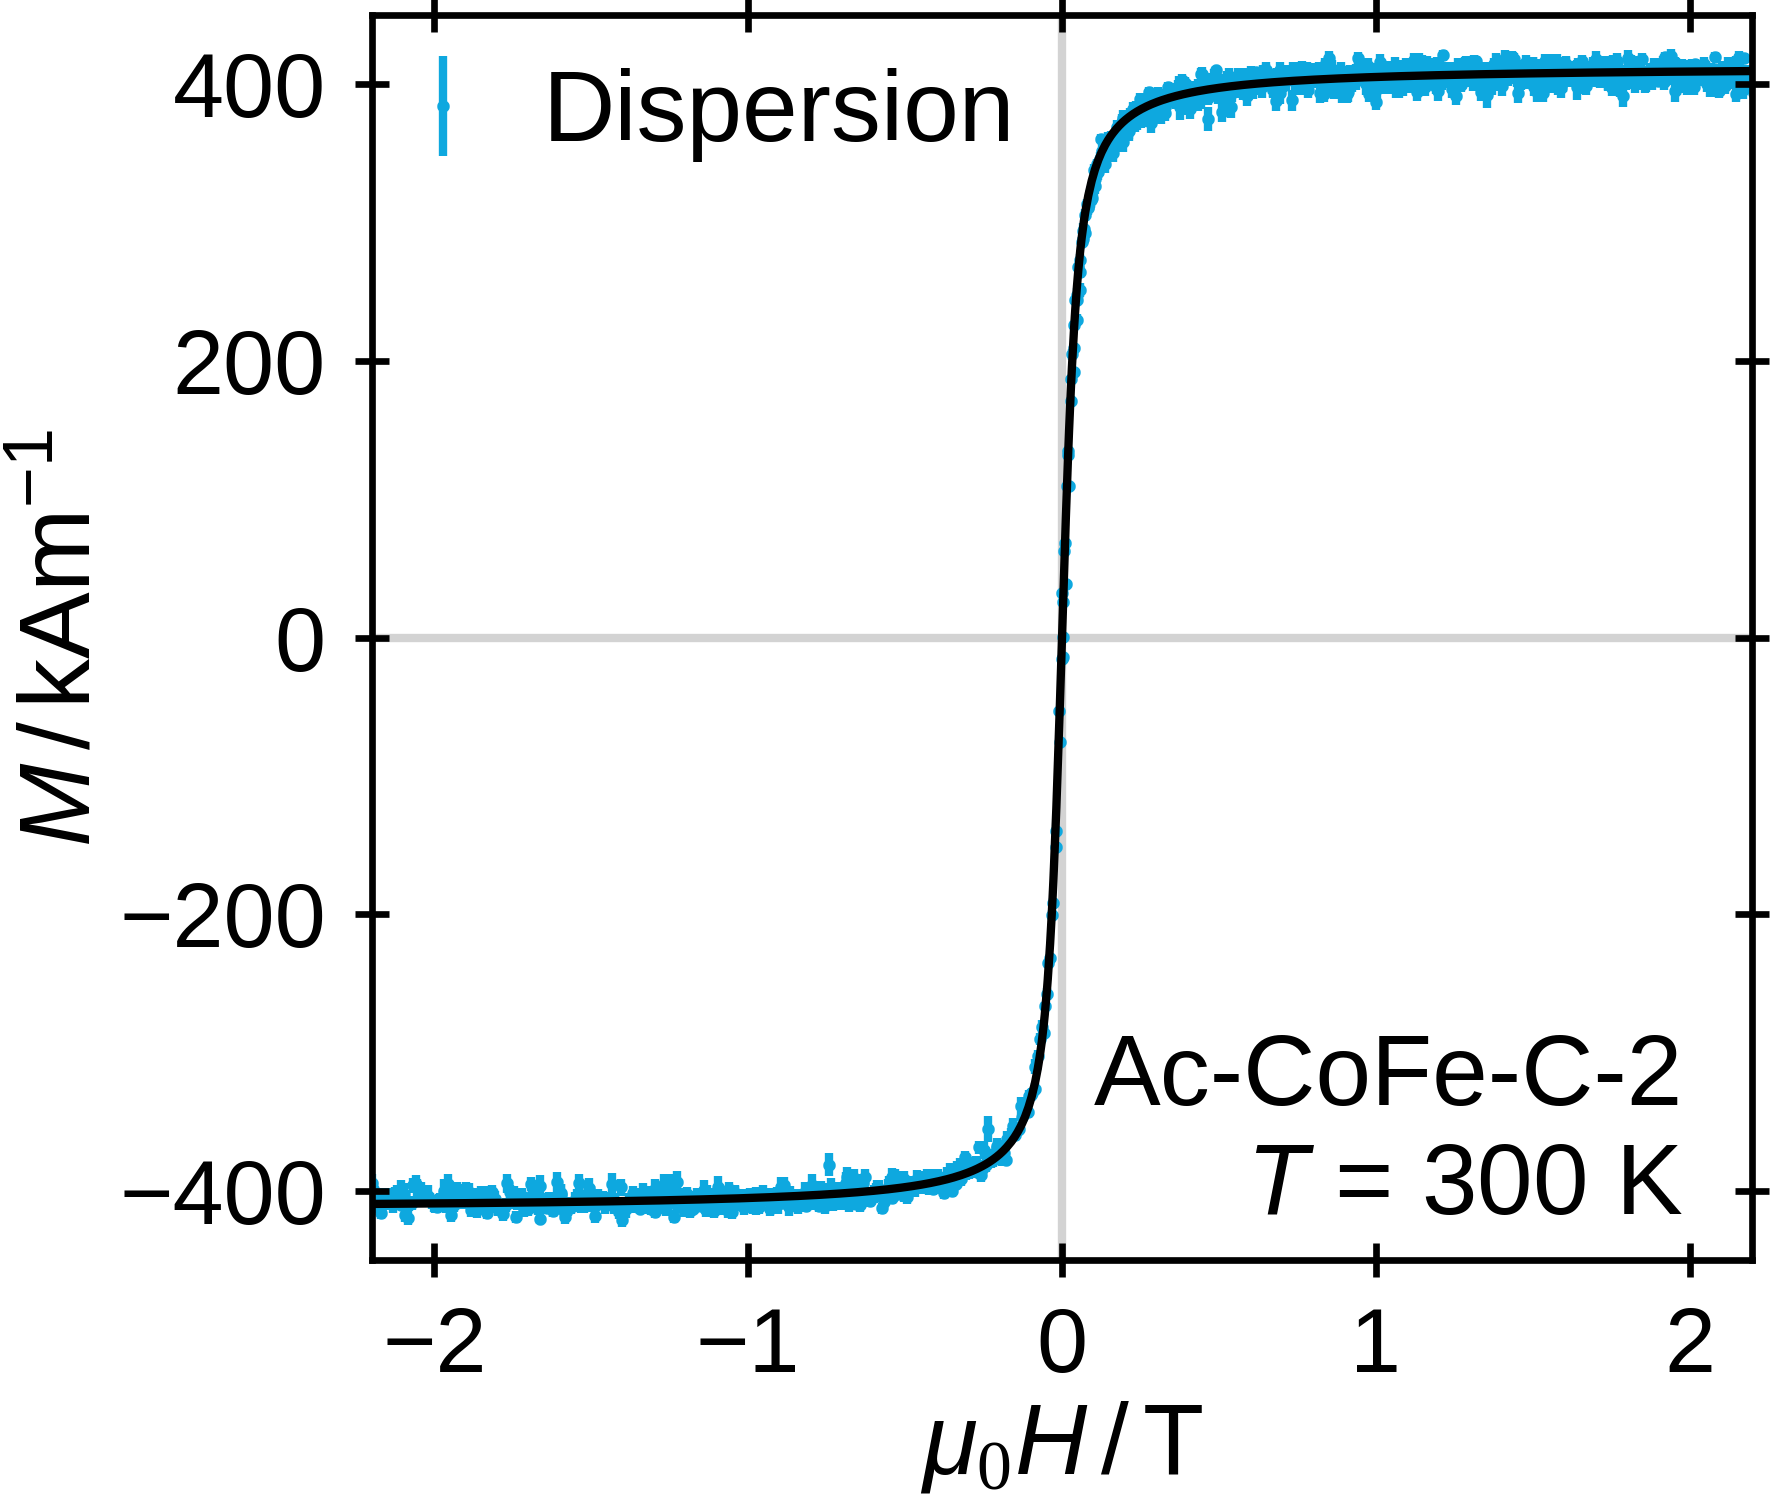
\includegraphics{monolayer_VSM_300K_Ac_CoFe_C_2}
    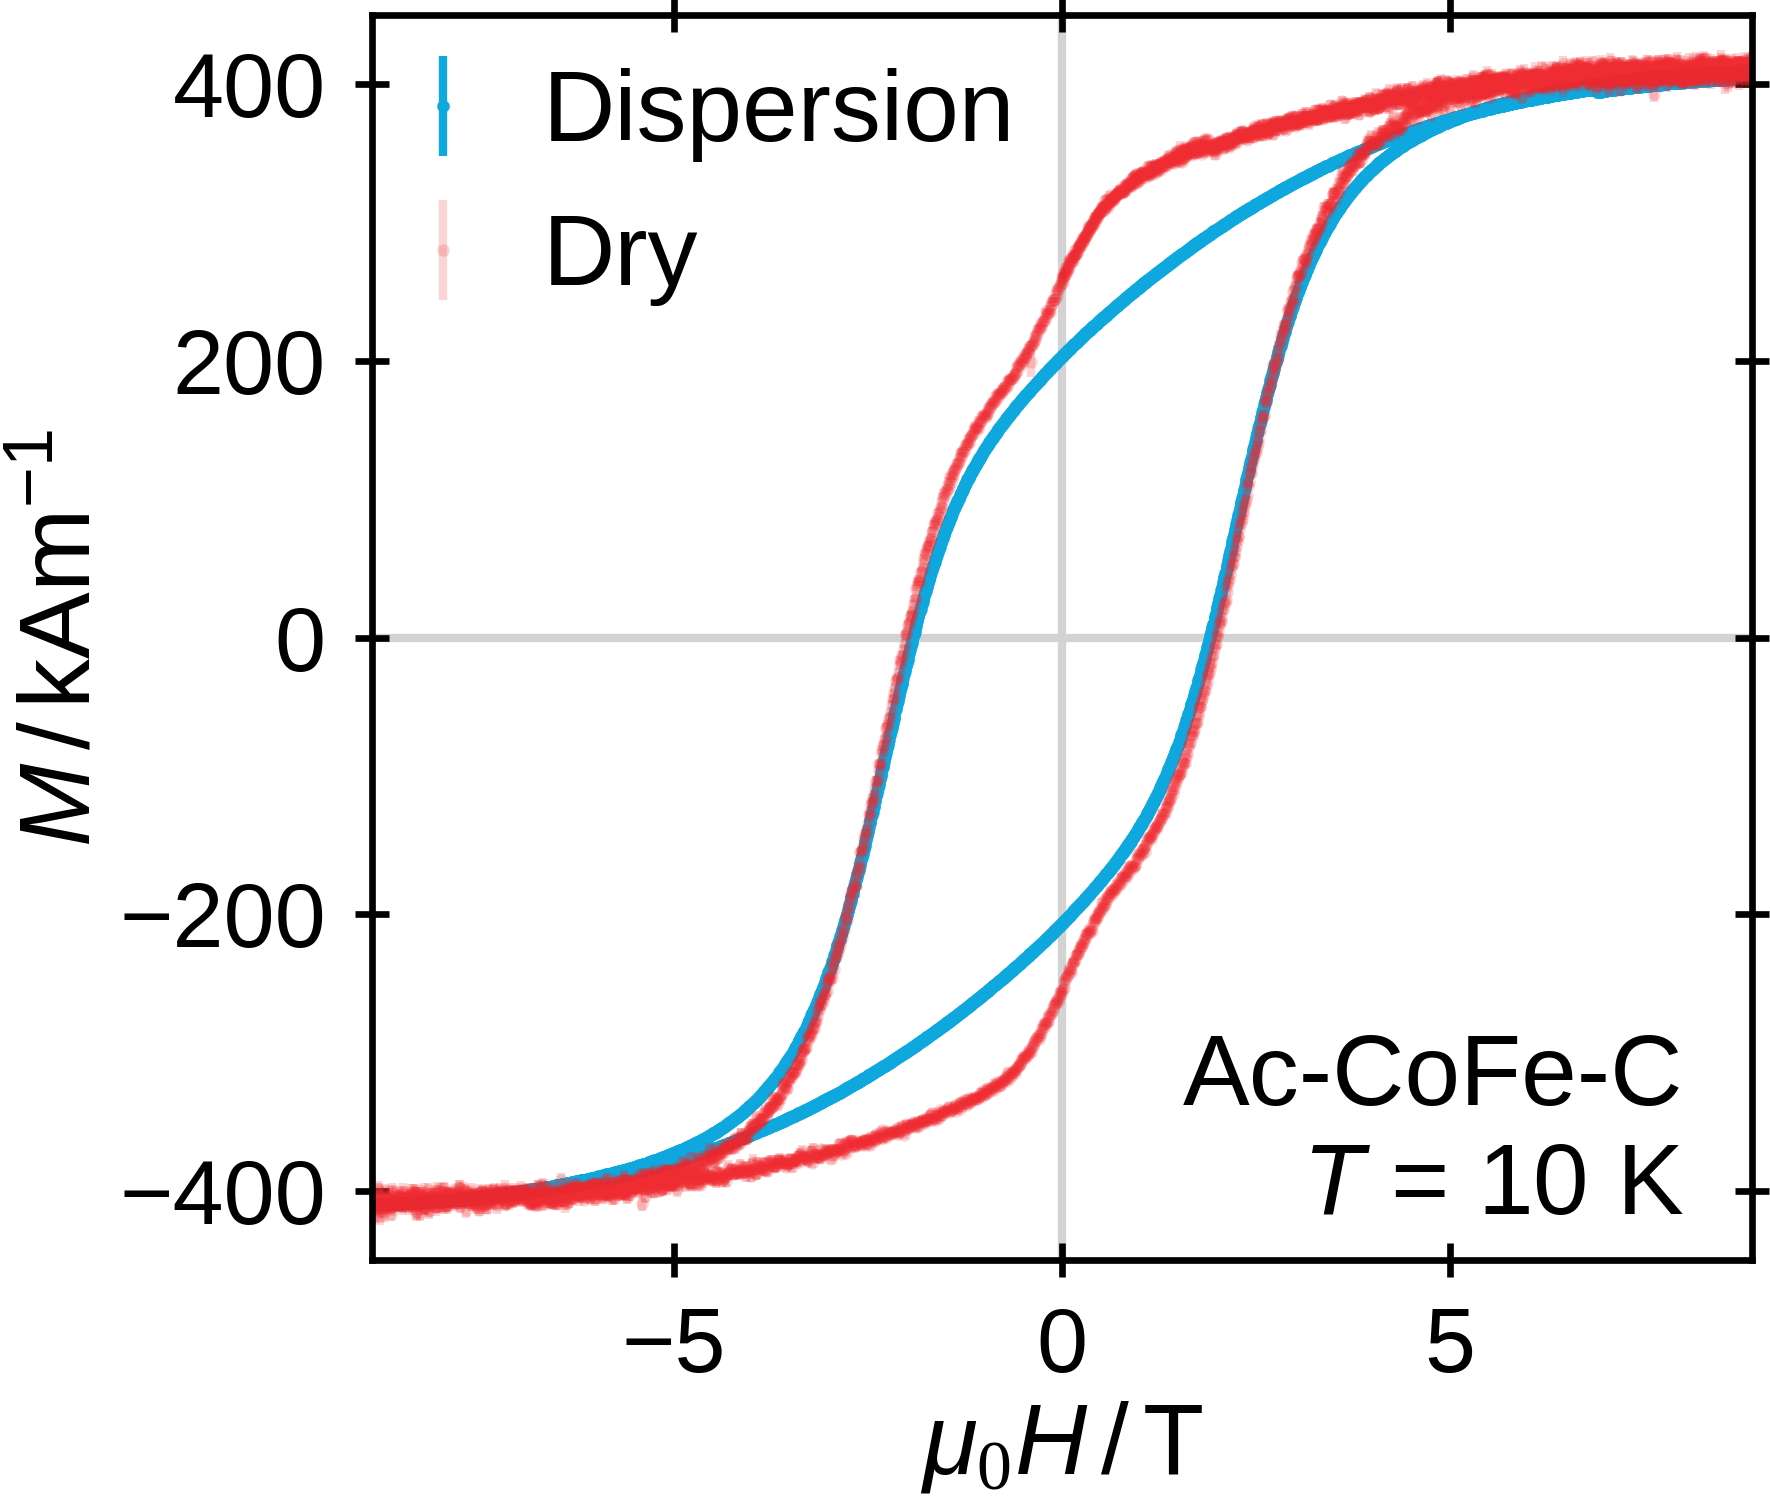
\includegraphics{monolayer_VSM_10K_Ac_CoFe_C_2}
    \caption{\label{fig:monolayers:nanoparticle:vsmAcCoFeC2}Field-dependent magnetization of Ac-CoFe-C-2 in dispersion measured at $300 \unit{K}$ (left) and $10 \unit{K}$ (right).}
  \end{figure}
  For Ac-CoFe-C-2 the dispersion in toluene has also been measured at $300 \unit{K}$ and $10 \unit{K}$ and are shown in \reffig{fig:monolayers:nanoparticle:vsmAcCoFeC2}.
  The same characteristics as for Ac-CoFe-C can be observed in the data.
  The magnetic moment at room temperature is determined to $23500(200) \mu_B$ and the coercive field at $10 \unit{K}$ also to $2.0 \unit{T}$.
  Although the magnetic moment is in the same order of magnitude as Ac-CoFe-C, due to the smaller nanoparticle size determined from small-angle scattering a higher spontaneous magnetization in the order of $M_s \eq 400 \unit{kA \, m^{-1}}$.

  \begin{figure}[tb]
    \centering
    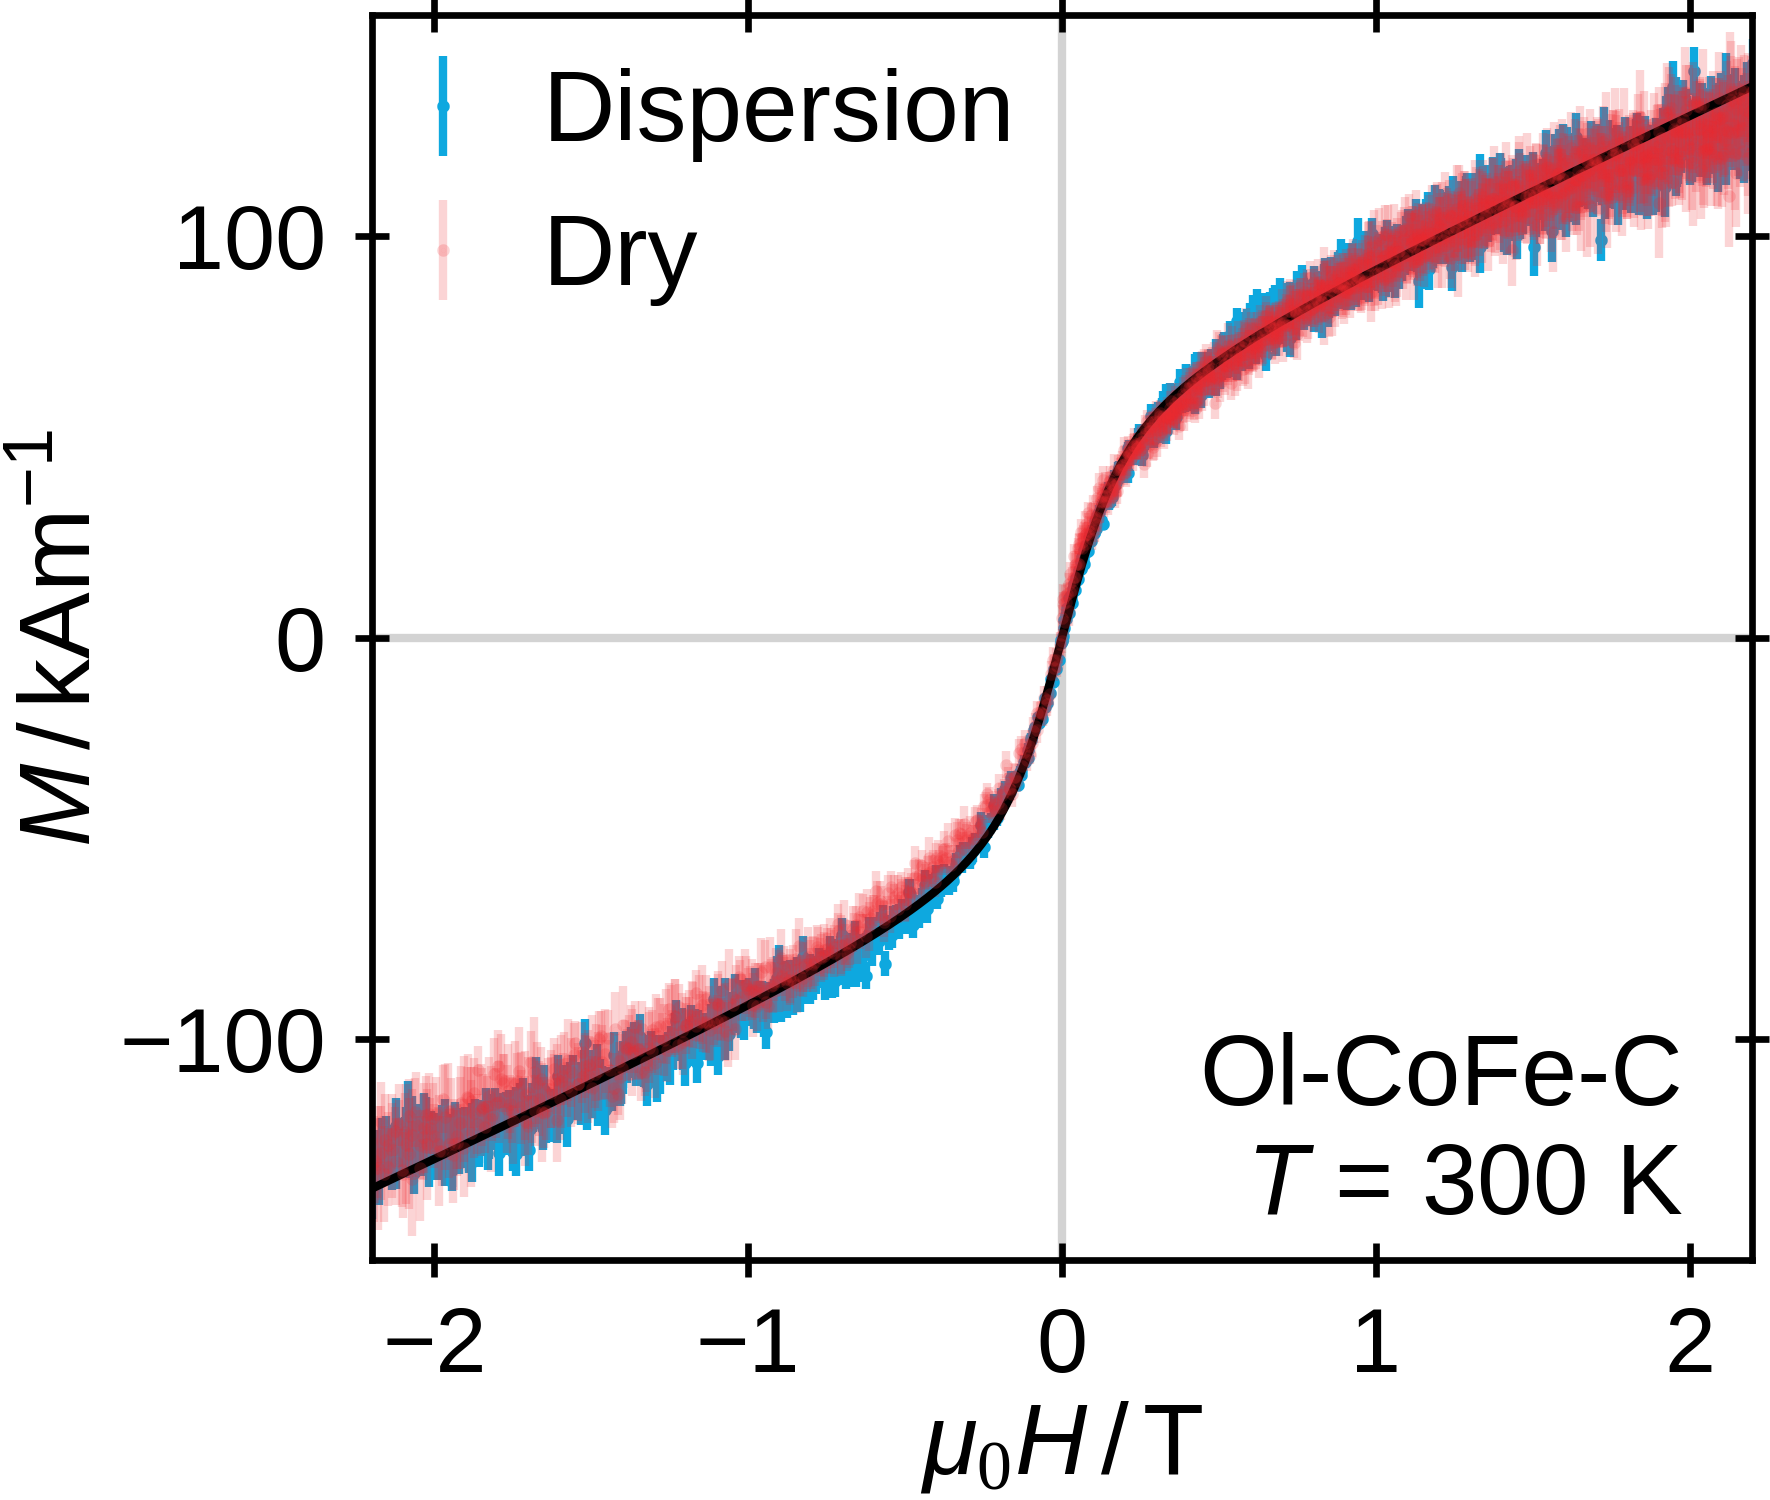
\includegraphics{monolayer_VSM_300K_Ol_CoFe_C}
    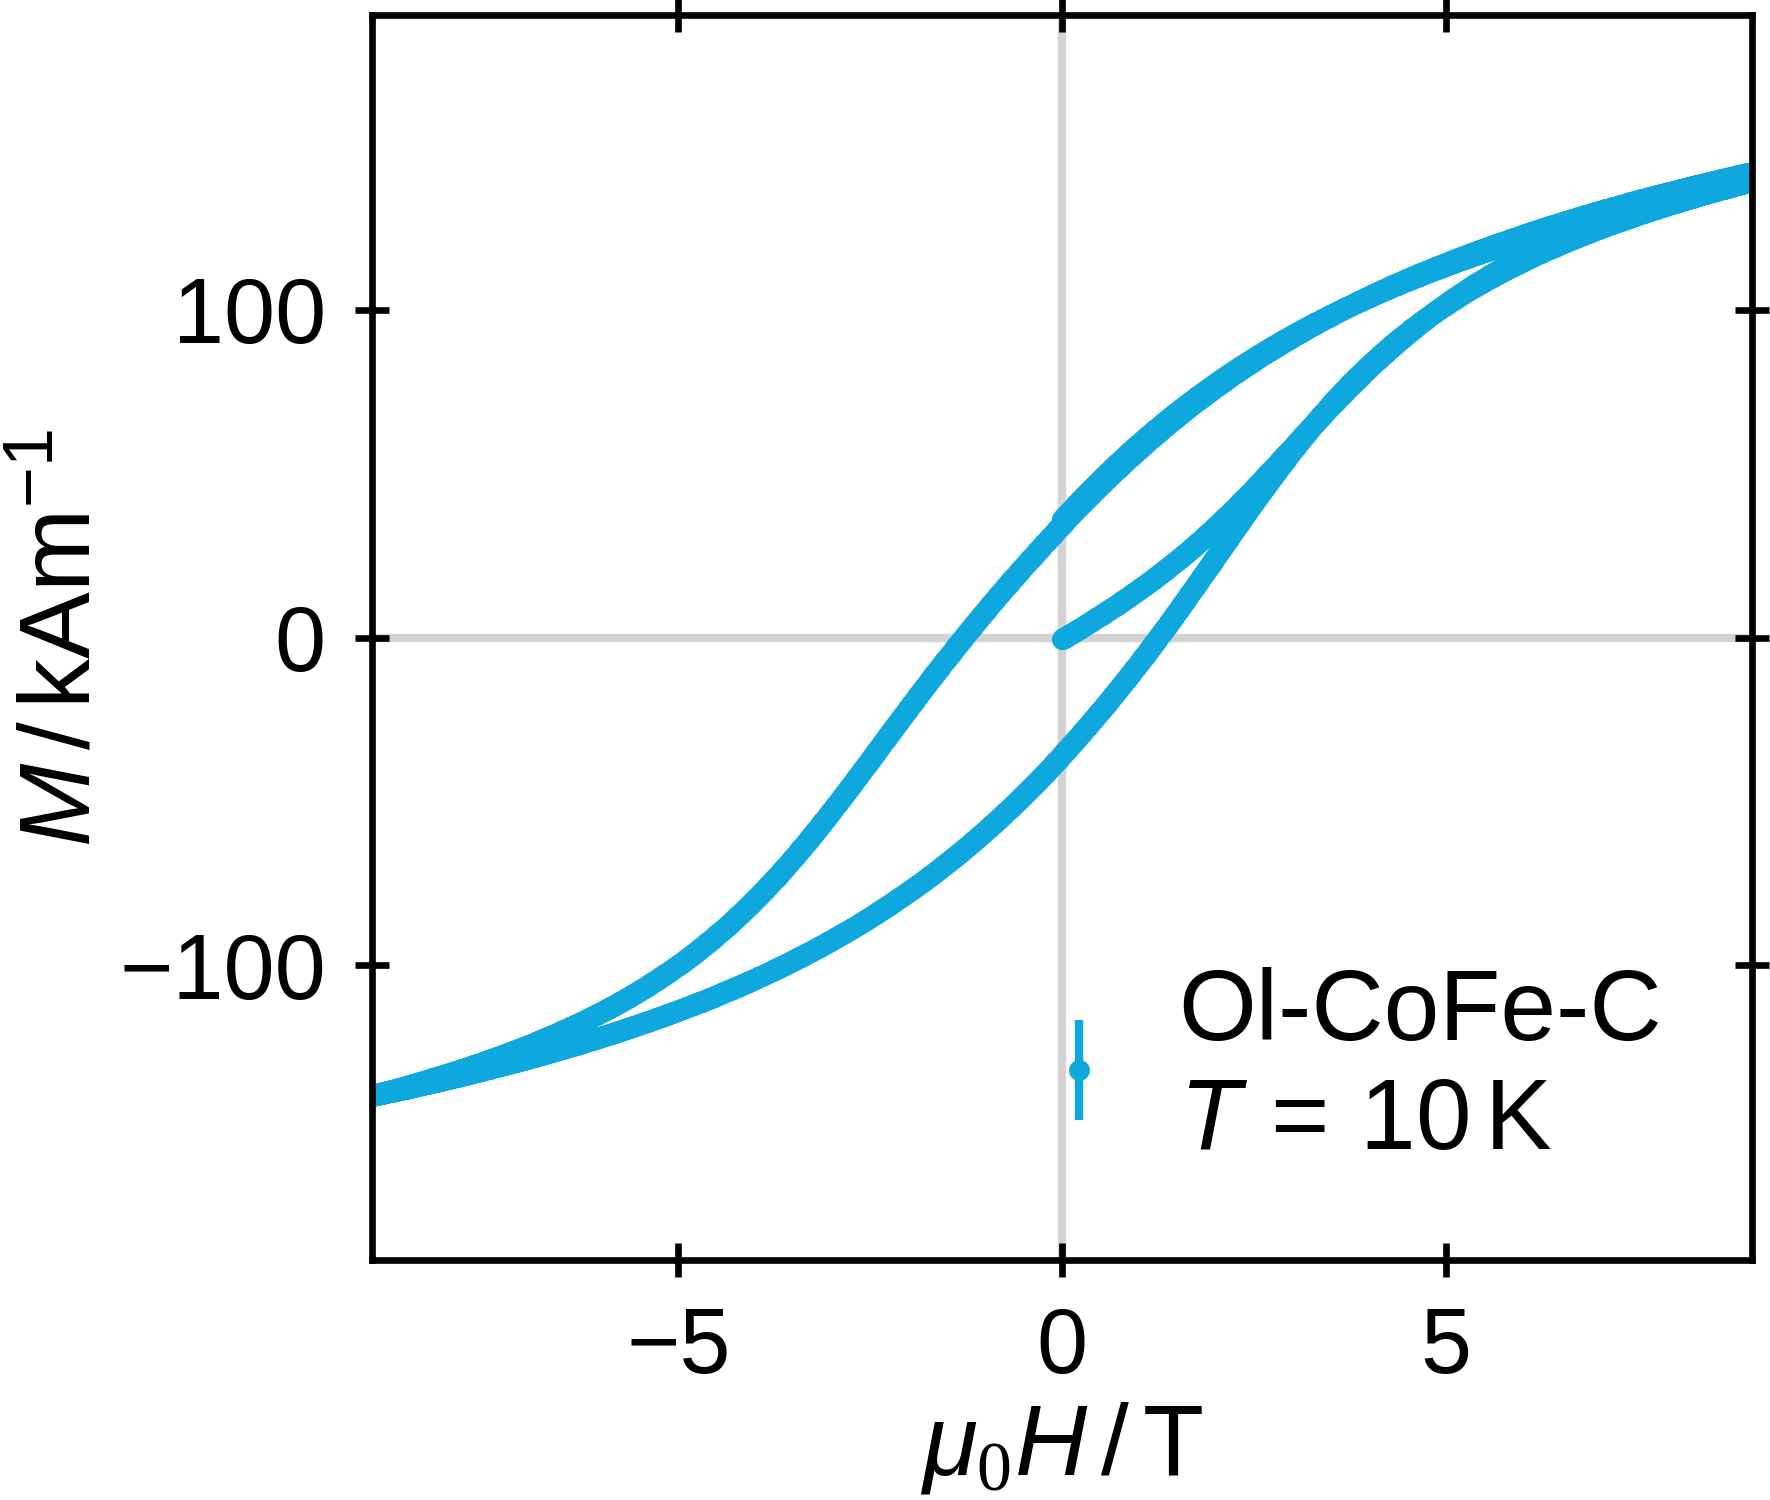
\includegraphics{monolayer_VSM_10K_Ol_CoFe_C}
    \caption{\label{fig:monolayers:nanoparticle:vsmOlCoFeC}VSM of Ol-CoFe-C at room temperature (left) and at $10 \unit{K}$ (right). The nanocubes are measured in dispersion and dried on a silicon substrate. The measurements in the dry state are corrected for the diamagnetic contribution from silicon.}
  \end{figure}

  Ol-CoFe-C shows a slightly different field-dependent magnetization behaviour visible in \reffig{fig:monolayers:nanoparticle:vsmOlCoFeC}.
  The measurement in dispersion and in the dry state both coincide at room temperature.
  From the fit of a Langevin behaviour with excess susceptibility results a magnetic moment of $6300(100) \mu_B$, a spontaneous magnetization of $57(1) \unit{kA \, m^{-1}}$ and an additional paramagnetic signal is visible as the sample does not saturate at high fields.
  The hysteresis shows a coercive field of $1.2 \unit{T}$ and is thus smaller than the coercivitiy of the Ac-CoFe-C nanocubes.
  A close inspection of the magnetization around $0 \unit{T}$ also shows a slight jump upon switching of the magnetic field direction, which is similar to the one observed in \reffig{fig:monolayers:nanoparticle:vsmAcCoFeC} and only smaller in magnitude.

  A temperature dependent measurement of the nanocubes Ol-CoFe-C on a substrate in \reffig{fig:monolayers:nanoparticle:vsm10K} (right) show a noisy signal due to the weak magnetization of the nanocubes and their low concentration.
  Using a median filter on the data, the underlying difference of the zero-field cooled and field cooled curve are visualized, from which a blocking temperature in the order of $210 \unit{K}$ is estimated.
  The value is smaller in comparison to the one observed from Ac-CoFe-C, which is connected to the core-shell structure of Ol-CoFe-C.
  As only the shell of the nanocubes Ol-CoFe-C is ferrimagnetic, the effective volume of the superparamagnetic nanoparticle is lower than the physical nanocube volume, which results in the lower blocking temperature.

  \begin{figure}[tb]
    \centering
    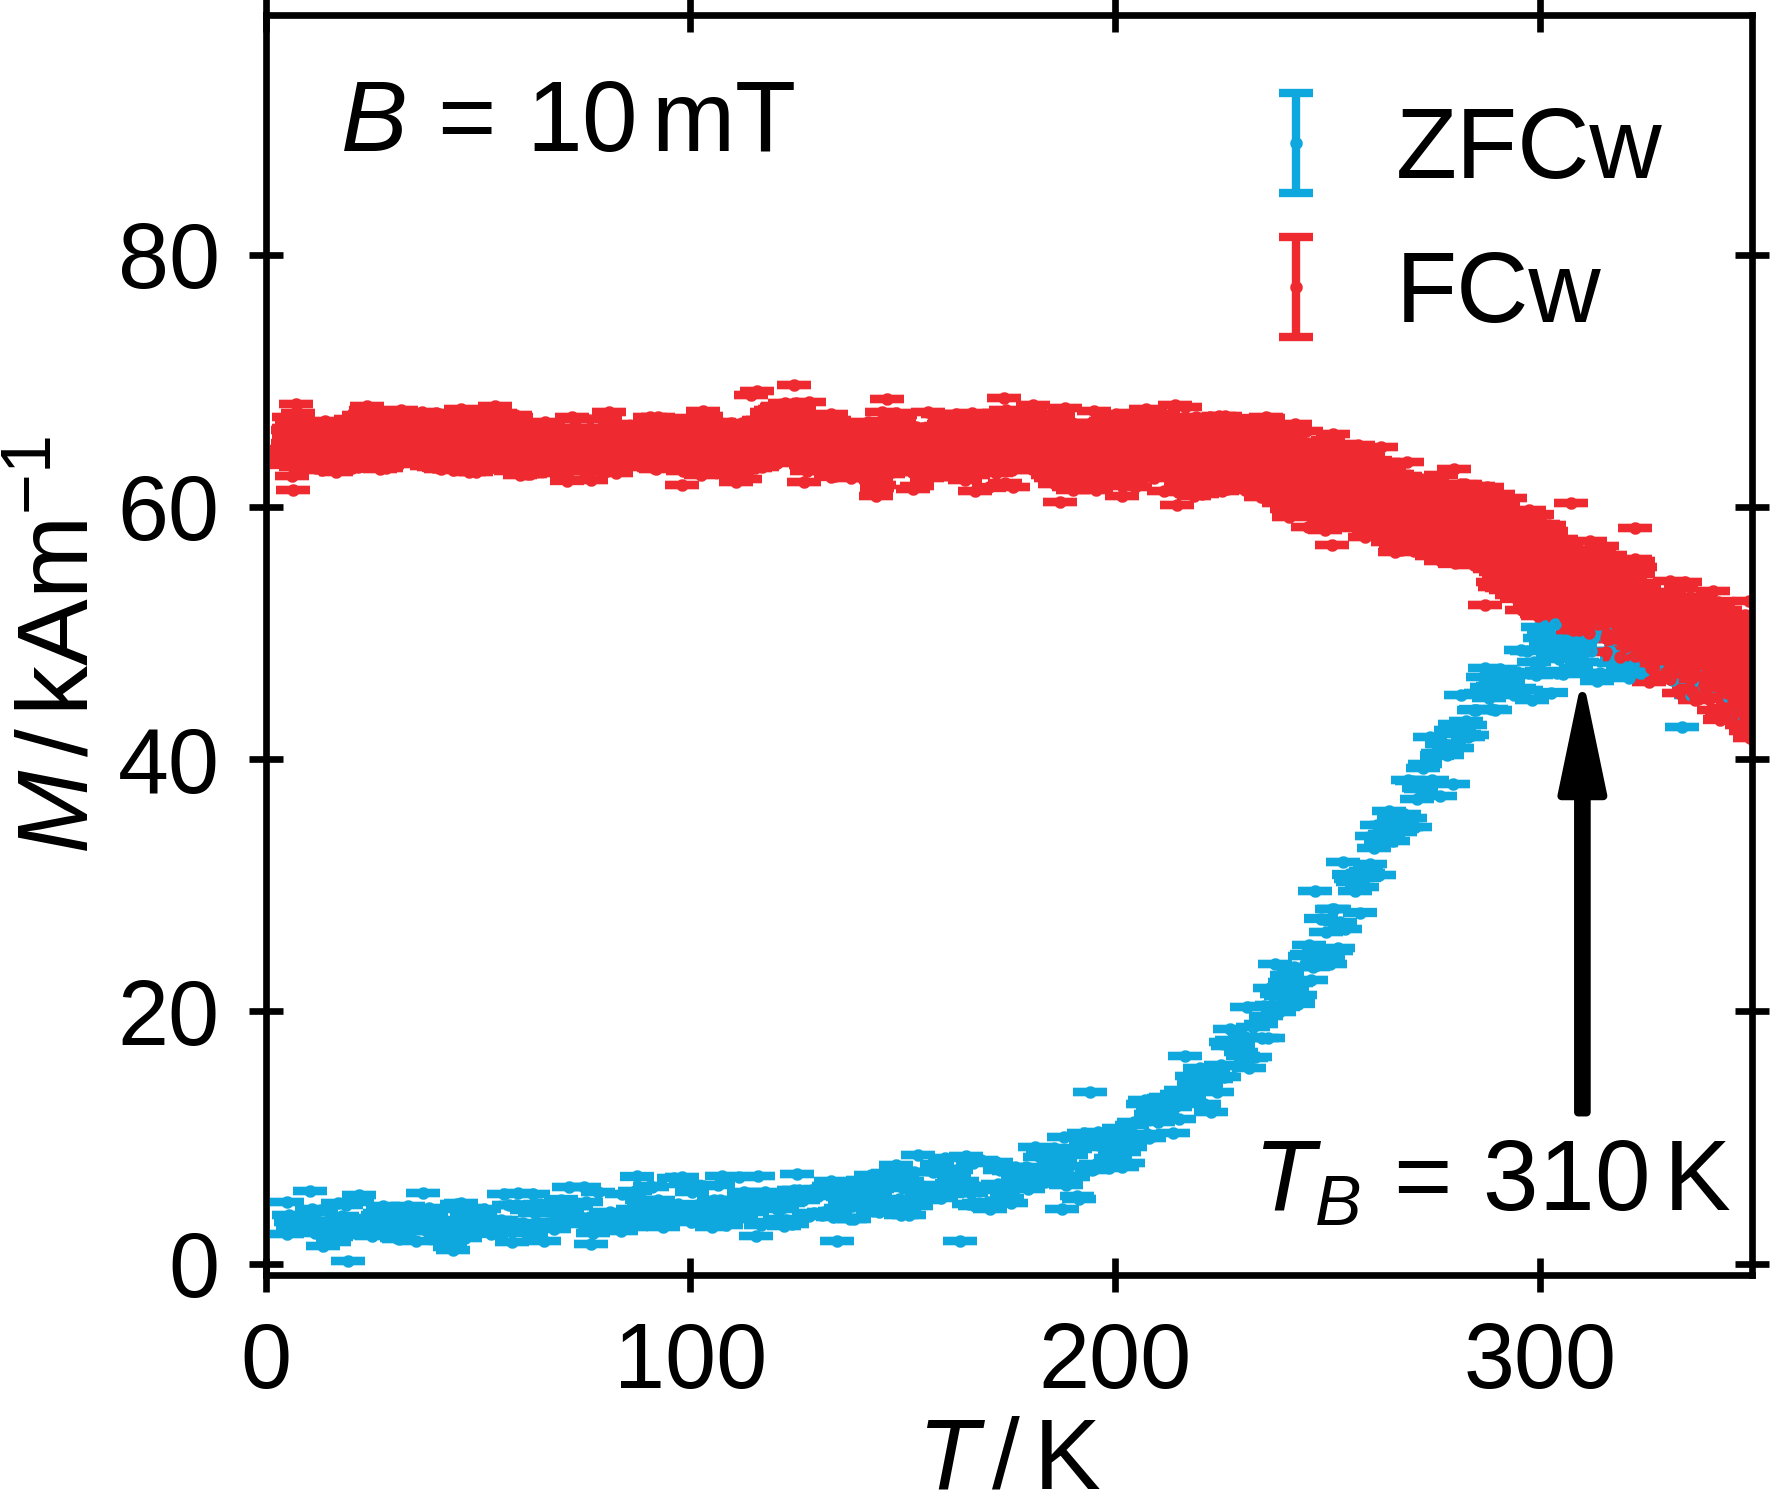
\includegraphics{monolayer_PPMS_ZFC_FC_ML_Ac_CoFe_C}
    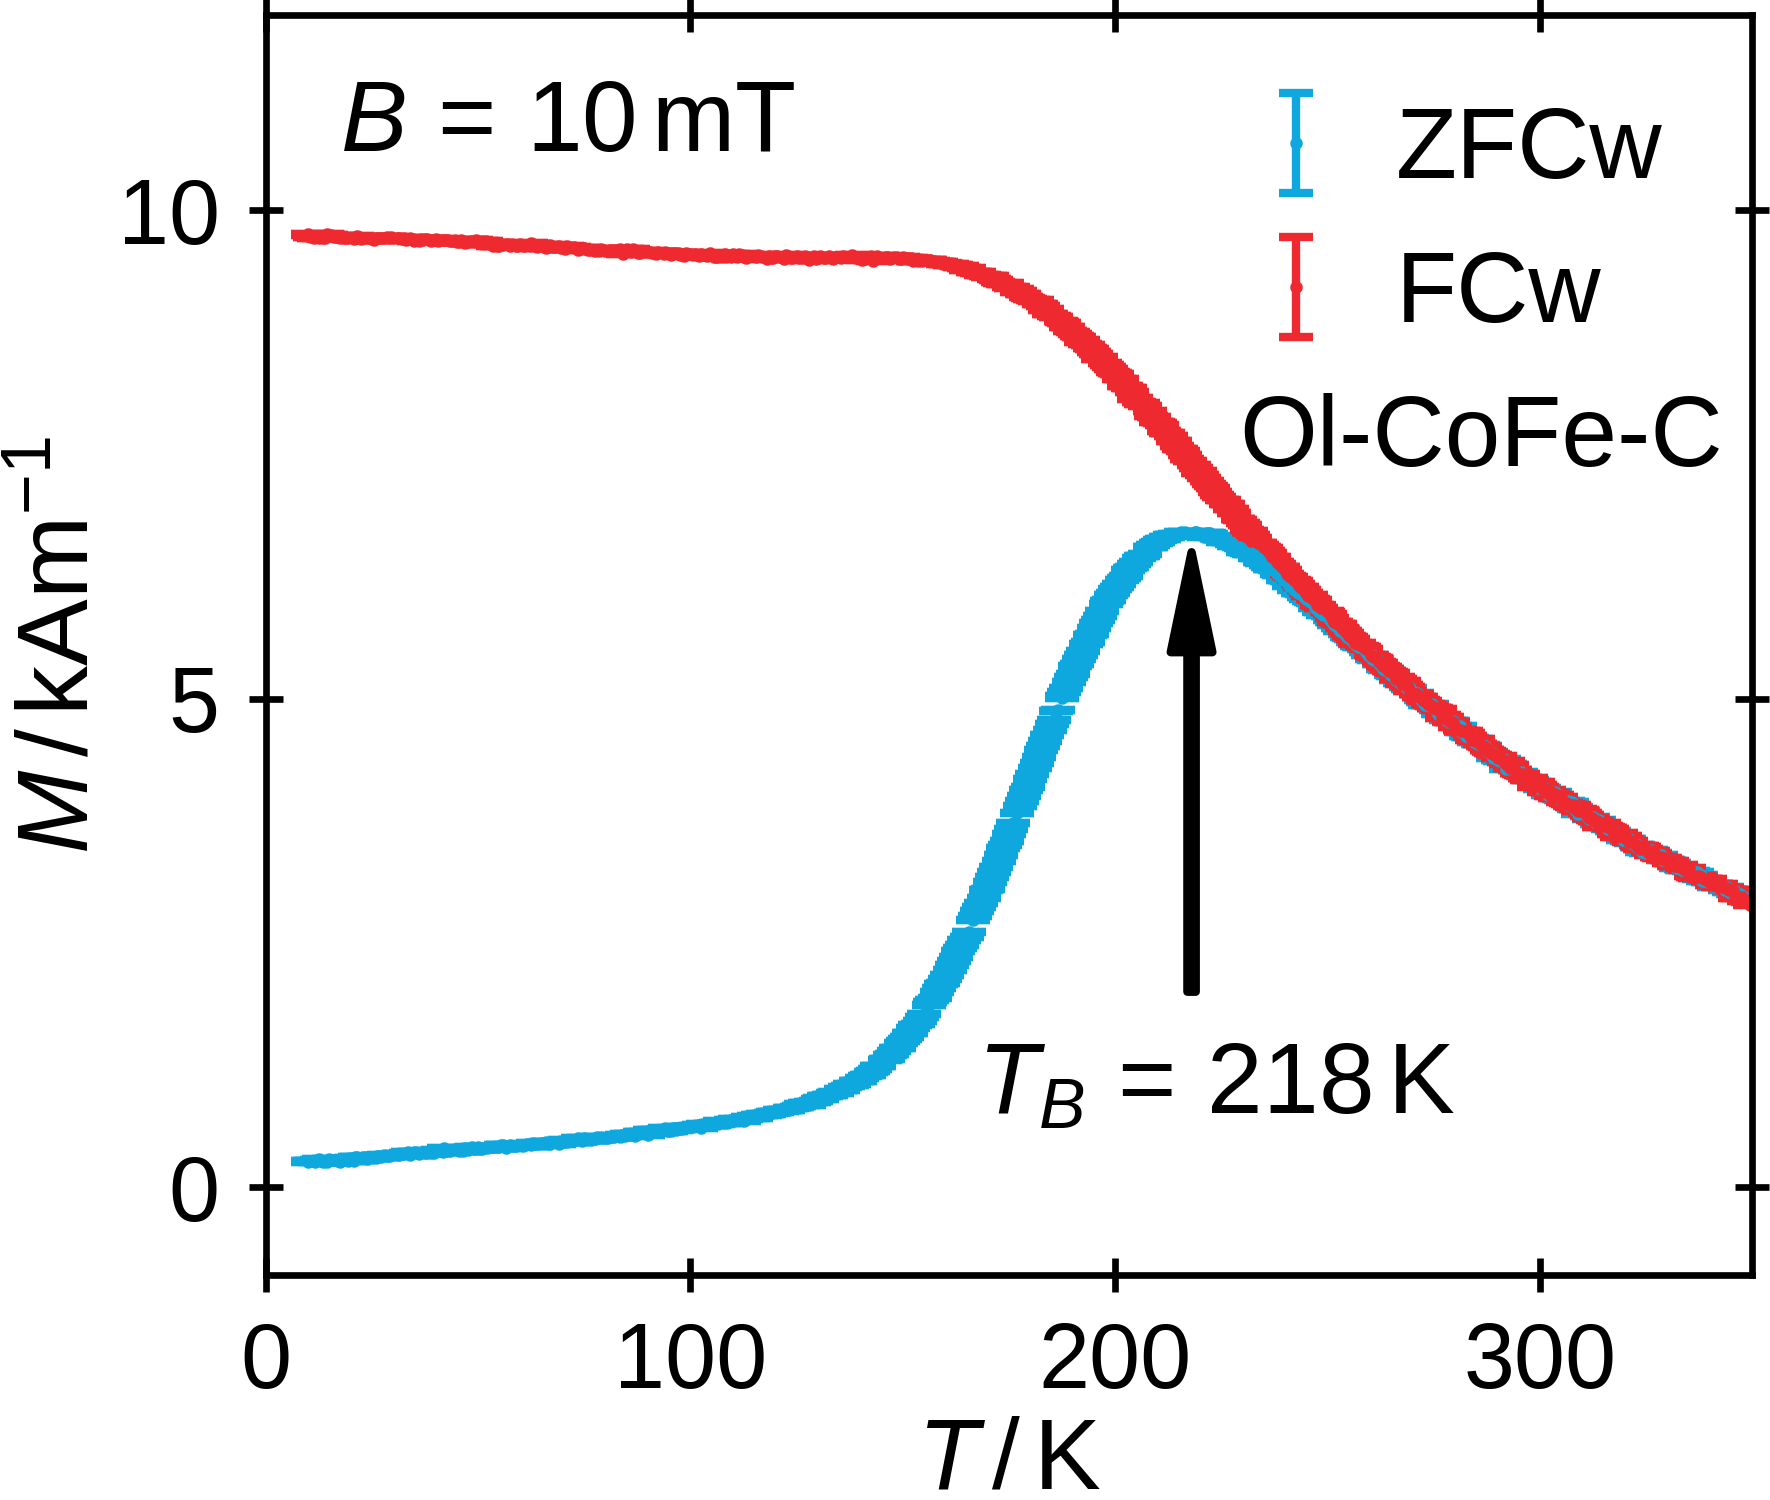
\includegraphics{monolayer_PPMS_ZFC_FC_ML_Ol_CoFe_C}
    \caption{\label{fig:monolayers:nanoparticle:vsm10K}Low temperature hysteresis measurement of frozen Ol-CoFe-C (left) and Ac-CoFe-C (right) using the same samples as in \reffig{fig:monolayers:nanoparticle:vsm}.}
  \end{figure}

\end{document}
